%!TeX root =  ../../thesis.tex

\section{UML}
\begin{figure}[h!]
	\centering
	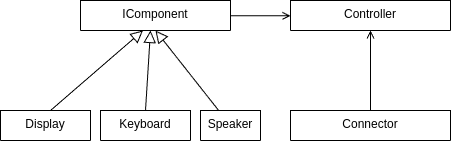
\includegraphics[width=0.9\textwidth]{pictures/diagram.png}
    	\caption{UML diagram tříd}
   	\label{fig:uml}
\end{figure}

Obrázek \ref{fig:uml} je UML diagram tříd. Třída Controller je hlavní třída, obsahuje kolekci Connectorů, ze kterých sice dědí konkrétní konektory, ale to je především pro přehlednost kódu, takže nebudu do diagramu uvádět všechny konkrétní konektory. Dále vidíme, že předek IComponent, který je abstraktní třídou, má tři potomky: Keyboard, Display a Speaker.